\documentclass{beamer}

% biber

\usepackage[brazilian]{babel}
\usepackage[utf8]{inputenc}
\usepackage{graphicx}
\usepackage{mathtools}
\usepackage{amsthm}
\usepackage{thmtools,thm-restate}
\usepackage{amsfonts}
\usepackage{amssymb}
\usepackage{hyperref}
\usepackage[backend=biber,url=true,doi=true,eprint=false,style=alphabetic]{biblatex}
\usepackage{enumitem}
\usepackage[justification=centering,singlelinecheck=false]{caption}
\usepackage{indentfirst}
\usepackage{tikz}
\usepackage{hyperref}
\usepackage{subcaption}
\usepackage{booktabs}
\usepackage{linegoal}
\usepackage{csquotes}
\usetikzlibrary{snakes,arrows,shapes}

\addbibresource{references.bib}

\setitemize{label=\usebeamerfont*{itemize item}%
  \usebeamercolor[fg]{itemize item}
\usebeamertemplate{itemize item}}

\setenumerate[1]{%
  label=\protect\usebeamerfont{enumerate item}%
        \protect\usebeamercolor[fg]{enumerate item}%
        \insertenumlabel.}

\uselanguage{brazilian}
\languagepath{brazilian}
\deftranslation[to=brazilian]{theorem}{teorema}
\deftranslation[to=brazilian]{Theorem}{Teorema}
\deftranslation[to=brazilian]{Definition}{Definição}
\deftranslation[to=brazilian]{definition}{definição}
\deftranslation[to=brazilian]{Lemma}{Lema}
\deftranslation[to=brazilian]{lemma}{lemma}
\deftranslation[to=brazilian]{Example}{Exemplo}
\deftranslation[to=brazilian]{example}{exemplo}
\usetheme{boxes}

\setbeamertemplate{bibliography entry title}{}
\setbeamertemplate{bibliography entry location}{}
\setbeamertemplate{bibliography entry note}{}

\setbeamertemplate{theorems}[ams style]

\DeclareMathOperator*{\argmin}{arg\,min}
\DeclareMathOperator*{\argmax}{arg\,max}
\DeclareMathOperator*{\Val}{\text{Val}}
\DeclareMathOperator*{\Ch}{\text{Ch}}
\DeclareMathOperator*{\Pa}{\text{Pa}}
\DeclareMathOperator*{\Sc}{\text{Sc}}
\DeclareMathOperator*{\PoA}{\text{PoA}}
\newcommand{\ov}{\overline}
\newcommand{\region}{\mathcal}

\captionsetup[table]{labelsep=space}

\theoremstyle{plain}

\newtheorem{proposition}{Proposição}
\newtheorem{exercise}{Exercício}

\newcommand{\set}[1]{\mathbf{#1}}
\newcommand{\pr}{\mathbb{P}}
\newcommand{\eps}{\varepsilon}
\renewcommand{\implies}{\Rightarrow}

\setlength{\parskip}{1em}

\newcommand{\code}[1]{\lstinline[mathescape=true]{#1}}
\newcommand{\mcode}[1]{\lstinline[mathescape]!#1!}

\newcommand{\p}{\pause}

\title{Jogos de Anti-Coordenação e Colorações Estáveis em Grafos}
\author{Renato Lui Geh\\NUSP:8536030}
\date{}

\begin{document}

\frame{\titlepage}

\section{Introdução}
\begin{frame}
  \frametitle{Introdução}

  \begin{block}{Jogos de coordenação:}
    Classe de jogos em que jogadores jogam cooperativamente. Jogador $i$ fazer a mesma ação que
    jogador $j$ gera um benefício para ambos jogadores.
  \end{block}\p

  \begin{block}{Exemplos:}
    \begin{itemize}
      \item Batalha dos sexos (visto em aula)\p
      \item Caça ao cervo
    \end{itemize}
  \end{block}
\end{frame}

\begin{frame}
  \begin{block}{Jogos de anti-coordenação:}
    Variante do jogo de coordenação em que jogador $i$ escolher mesma ação que jogador $j$ gera
    custo.
  \end{block}\p

  \begin{block}{Exemplos:}
    \begin{itemize}
      \item Mineração\p
      \item Habilidades de empregados\p
      \item Rotas de avião
    \end{itemize}
  \end{block}
\end{frame}

\begin{frame}
  \begin{block}{Dois jogadores:}
    \begin{itemize}
      \item Fácil
      \item Matriz de utilidade/custo
    \end{itemize}
  \end{block}\p

  \begin{block}{Mais de dois jogadores:}
    \begin{itemize}
      \item Difícil
      \item Grafos
    \end{itemize}
  \end{block}
\end{frame}

\begin{frame}
  \textbf{Jogo:} $G=(V,E)$\\
  \begin{align*}
    v\in V:\quad &\text{jogador}\\
    e\in E:\quad &\text{relação entre dois jogadores}\\
    \{1,\ldots,k\}:\quad &\text{ações}\\
  \end{align*}
  \textbf{Utilidade:} número de vizinhos que têm ações diferentes\\
  \textbf{Equilíbrio:} $v$ não tem incentivo para mudar ação dados vizinhos\p\\~\\

  Parece com algo? \p \textbf{Coloração}
\end{frame}

\begin{frame}
  \frametitle{Objetivos:}
  \begin{enumerate}
    \item Para $k\geq 2$, existe algoritmo polinomial para achar $k$-coloração estável num grafo
      não-direcionado.\p
    \item PoA para $k$-coloração em grafos não-direcionado é $\Theta\left(\frac{k}{k-1}\right)$.\p
    \item Para $k\geq 2$, descobrir se existe $k$-coloração estritamente estável num grafo
      não-direcionado é NP-difícil.\p
  \end{enumerate}

  Existe generalização do 3 para digrafos, mas vou mostrar apenas para grafos não-direcionados.
  Vejam~\cite{kun-et-al} se estiverem curiosos.
\end{frame}

\section{Definições}

\begin{frame}
  \frametitle{Definições}
  Seja $G=(V,E)$ grafo não-direcionado.\\
  Chamamos $c\in C=\{f|f:V\to\{1,\ldots,k\}\}$ de uma coloração.\\~\\

  Todos $v\in V$ escolhem cor simultaneamente. A utilidade de $v$ é:

  \begin{equation*}
    \mu_c(v) \coloneqq \sum_{\{u,v\}\in E} 1_{\{c(u)\neq c(v)\}}
  \end{equation*}

  O valor social de $G$ dada uma coloração $c$ é:

  \begin{equation*}
    W(G,c)\coloneqq\sum_{v\in V}\mu_c(v)
  \end{equation*} 
\end{frame}

\begin{frame}
  Uma coloração $c$ é \textbf{estável} se nenhum vértice $v$ pode aumentar $\mu_c(v)$ mudando
  $c(v)$.\p\\~\\

  Uma coloração $c$ é \textbf{estritamente estável} se para todo $v\in V$, toda $c'\in C$, $c'\neq
  c$ temos que $\mu_c(v)>\mu_{c'}(v)$. Senão, $c$ é \textbf{não-estrita}.\p\\~\\

  O PoA de $G$ é:

  \begin{equation*}
    \PoA(G)\coloneqq\frac{\max_{c'\in C} W(G,c')}{\min_{c\in Q} W(G,c)}
  \end{equation*}

  onde $Q$ é o conjunto de colorações estáveis.
\end{frame}

\begin{frame}
  \begin{figure}[h]
    \centering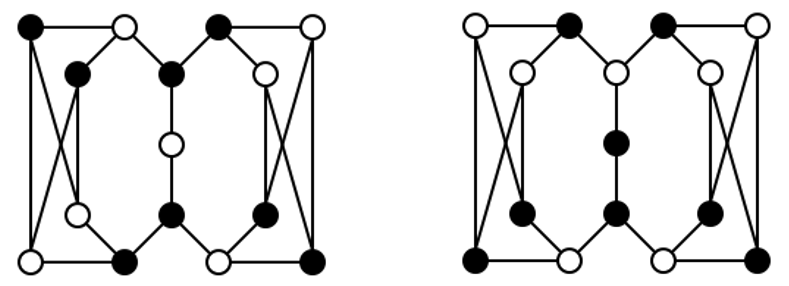
\includegraphics[scale=0.3]{imgs/ex1.png}
    \captionsetup{justification=raggedright}
    \caption{O grafo da esquerda é estritamente estável e tem $W(G,c)=40$, enquanto que o da
    direita é não-estrito com $W(G,c')=42$. Fonte:~\cite{kun-et-al}}
  \end{figure}
\end{frame}

\begin{frame}
  \frametitle{Colorações estáveis}
  \begin{proposition}\label{prop-1} Para todo $k\geq 2$, todo grafo finito $G=(V,E)$ admite uma
    $k$-coloração estável. Tal $k$-coloração estável pode ser encontrada em tempo polinomial.
  \end{proposition}
\end{frame}

\begin{frame}
  \frametitle{Demonstração (Proposição 1)}
  Primeiro chamaremos:
  \begin{align*}
    c:\quad &\text{coloração}\\
    \phi(c):\quad &\text{número de arestas coloridas apropriadamente}
  \end{align*}\p
  Note que $0\leq \phi(c)\leq |E|$. Vamos primeiro mostrar que $W(G,c)=2\phi(c)$.\\~\\\p
  Fixa $v\in V$.\p
  \begin{align*}
    &n_v:\quad \text{número de cores diferentes em $v$}\\
    &\phi(c)=\sum_{e\in E}1_{\{e\text{ apropriado}\}}
  \end{align*}\p
  Se $e$ é apropriado ($c(u)\neq c(v)$), então contamos $e$ duas vezes: $(u,v)$ e $(v,u)$.
\end{frame}

\begin{frame}
  Somando todas as arestas apropriadas para todo $v$:
  \begin{equation*}
    \sum_{v\in V}\sum_{e=\{u,v\}\in E}1_{\{e\text{ apropriado}\}}=\sum_{v\in V}n_v=2\phi(c)
  \end{equation*}\p
  Mas $n_v$ é exatamente $\mu_c(v)$.\p
  \begin{equation*}
    \sum_{v\in V}n_v=2\phi(c)=\sum_{v\in V}\mu_c(v)=W(G,c)
  \end{equation*}\p
  Note que $\phi(c)$ é uma função potencial exata, então esse é um jogo de potencial.
\end{frame}

\begin{frame}
  Dada uma coloração $c$, um vértice $v$ está \textit{infeliz} se $v$ tem mais vizinhos com mesma
  cor que $v$ do que diferentes.\p

  Para acharmos uma $k$-coloração estável em $G$ fazemos:

  Enquanto existe algum vértice $v$ infeliz, mude $c(v)$ para algum $c'(v)$ tal que
  \begin{equation*}
    c'(v)=\argmin_{m\in\{1,\ldots,k\}}\sum_{u\in N(v)}1_{\{c(u)=m\}},
  \end{equation*}
  onde $N(v)$ são os vizinhos de $v$.
\end{frame}

\begin{frame}
  Se $v$ é vértice infeliz, então mudar para $c'(v)$ vai sempre aumentar $\phi$. Aumentar $\phi$
  aumenta $W(G,c)$, pois $W(G,c)=2\phi$.

  Como a cada iteração pelo menos uma aresta vai ser colorida de forma a aumentar $\phi$, então
  depois de no máximo $|E|$ iterações, nenhum $v\in V$ estará infeliz.

  Se nenhum vértice está infeliz, então nenhum vértice terá incentivo para mudar. Então a coloração
  é estável.

  \hfill$\qed$
\end{frame}

\begin{frame}
  \begin{proposition}
    O preço da anarquia de uma $k$-coloração de um jogo de anti-coordenação é $\Theta\left(
    \frac{k}{k-1}\right)$.
  \end{proposition}
\end{frame}

\begin{frame}
  \frametitle{Demonstração (Proposição 2)}
  Existem $k$ cores. Fixe vértice $v$ e coloração $c$. A utilidade $\mu_c(v)$ pode ser no máximo
  $k-1$.

  \textbf{Princípio da casa dos pombos (PCP):} $n=l\cdot m+1$ objetos distribuídos em $m$
  conjuntos, então pelo menos um conjunto terá $l+1$ objetos.

  Pelo PCP, todo vértice $v$ pode alcançar pelo menos $\frac{k-1}{k}\cdot\deg(v)$ usando o
  algoritmo da Proposição 1. Então

  \begin{equation*}
    \PoA(G)=\frac{\max_{c'\in C} W(G,c')}{\min_{c\in Q}W(G,c)}=\frac{\sum_{v\in
      V}\deg(v)}{\sum_{v\in V}\frac{k-1}{k}\cdot\deg(v)}=\frac{k}{k-1}
  \end{equation*}

  é o PoA máximo.
\end{frame}

\begin{frame}
\end{frame}

%--------------------------------------------------------------------------------------------------

\section[Referências]{Referências e Bibliografia}
\begin{frame}[t,allowframebreaks]
  \frametitle{Referências e Bibliografia}
  \nocite{*}
  \printbibliography[]
\end{frame}

\end{document}
